\documentclass[titlepage]{article}
\usepackage[czech]{babel}
\usepackage{pdfpages}
\usepackage{amsmath}
\usepackage{pgfplots}
\usepackage{siunitx}
\usepackage[parfill]{parskip}
\usepackage{float}
\usepackage{hyperref}
\hypersetup{
    colorlinks,
    citecolor=black,
    filecolor=black,
    linkcolor=black,
    urlcolor=black
}
\sisetup{detect-all}

\begin{document}
%opening
\begin{titlepage}
 \includepdf{razitko.pdf}
\end{titlepage}

\tableofcontents
\newpage

\section{Úkol měření}

\begin{enumerate}
 \item Na základě měření vnějšího fotoelektrického jevu ověřte velikost Planckovy konstanty $h$.
 \item Určete výstupní práci materiálu fotokatody použité fotonky. Porovnejte tuto hodnotu s výstupními pracemi jiných materiálů a odhadněte, z jakého materiálu je tato fotokatoda vyrobena.
 \item Určete nejistotu měření pro všechny veličiny určené v bodech 1 a 2.
 \item Vypracujte graf závislosti maximální kinetické energie elektronů na frekvenci záření $W_k = f(\nu)$.
 \item Změřte závislost fotoelektrického proudu na velikosti brzdného potenciálu pro dvěvlnové délky.
 \item Do jednoho grafu vyneste pro obě vlnové délky změřené závislosti fotoelektrického proudu na velikosti brzdného potenciálu.
 \item Porovnejte hodnotu změřené Planckovy konstanty s tabulkovou hodnotou a rozdíl zhodnoťte.
 \item Měření a zpracování dat v bodech 1-7 proveďte zvlášť pro obě instalované měřící aparatury, závislosti $W_k= f(\nu)$ vyneste do jednoho (společného) grafu. Body 5-6 provádějte pouze pro soupravu se spektrálním fotometrem Spekol.
\end{enumerate}

\section{Seznam použitých přístrojů}
\begin{itemize}
 \item Soustava se spektrálním fotometrem Spekol
 \begin{itemize}
  \item Nejmenší dílek stupnice pro měření proudu: $1 \si{\micro\ampere}$
  \item Nejmenší dílek stupnice pro nastavení vlnové délky světla: $1 \si{\nano\meter}$
 \end{itemize}

 \item Multimetr MY-64
 \begin{itemize}
  \item rozsah $2 \si{\volt}$, přesnost $\pm 0.5 \%$ z údaje $\pm 1$ digit
 \end{itemize}


 \item Multimetr MY-65
 \begin{itemize}
  \item rozsah $2 \si{\volt}$, přesnost $\pm 0.1 \%$ z údaje $\pm 1$ digit
  \item rozsah $200 \si{\milli\volt}$, přesnost $\pm 0.05 \%$ z údaje $\pm 3$ digit
 \end{itemize}

 \item Souprava svýbojkou a monochromatickými filtry
\end{itemize}

\section{Teoretický úvod}
\subsection{Stanovení Planckovy konstanty}
Fotony při dopadu na kovy předávají svoji energii elektronům v kovu. Tento jev je popsán Einsteinovou rovnicí pro fotoefekt
\begin{equation}\label{eq:einstein}
 h\nu = \frac{1}{2}mv^2 + A = W_k + A
\end{equation}
Kde je energie fotonu dána součinem Planckovy konstanty $h$ a frekvence $\nu$. Tato energie se poté dělí na kinetickou energii elektronu $W_k = \frac{1}{2}mv^2$, kde $m$ je hmotnost elektronu a $v$ jeho rychlost, a výstupní práci $A$, což je energii potřebná k překonání potenciálové bariéry kovu. Pro tuto frekvenci platí
\begin{equation}
 \nu = \frac{c}{\lambda}\label{eq:frequency}
\end{equation}
kde $c = 2.99792458 \cdot 10^8 \si{\meter\per\second}$ je rychlost světla a $\lambda$ vlnová délka světla.

Pokud v kovu vytvoříme elektrické pole, které emitované elektrony zabrzdí, tedy proud v něm bude nulový, pak platí, že kinetická energie elektronů $W_k$ je rovna potenciální energii, která je brzdila, tedy
\begin{equation}\label{eq:energy}
 W_k = \frac{1}{2}mv^2=eU_p
\end{equation}
kde$U_p$ je napětí, při němž došlo k vykompenzovaní a $ e = 1.602 \cdot 10^{-19} \si{\coulomb}$ je velikost náboje elektronu.

\subsubsection{Použití metody nejmenších čtverců}
Upravíme-li vztah \eqref{eq:einstein} dostaneme
\begin{equation}
 W_k = h\nu - A
\end{equation}
Tento vztah aproximujeme přímkou ve tvaru
\begin{equation}\label{eq:squares}
 W_k = a_1\nu+a_0
\end{equation}
Nyní dostáváme odhady
\begin{equation}\label{eq:work}
 A = -a_0
\end{equation}
\begin{equation}\label{eq:planck}
 h = 1.602 \cdot 10^{-19}a_1
\end{equation}

\newpage
\section{Naměřené hodnoty a jejich zpracování}
\subsection{Tabulky naměřených hodnot}
\subsubsection{Závislost veliksoti brzdného napětí na vlnové délce}
\begin{table}[!htb]
    \begin{minipage}{.5\linewidth}
      \centering
        \begin{tabular}{c||c}
           $\lambda [\si{\nano\meter}]$ & $U_p [\si{\volt}]$\\ \hline \hline
           375 & 1.215\\ \hline
           400 & 1.057\\ \hline
           425 & 0.981\\ \hline
           450 & 0.854\\ \hline
           475 & 0.757
        \end{tabular}
        \caption{Přístroj Spekol}
    \end{minipage}%
    \begin{minipage}{.5\linewidth}
      \centering
        \begin{tabular}{c||c}
           $\lambda [\si{\nano\meter}]$ & $U_p [\si{\volt}]$\\ \hline \hline
           408 & 1.039\\ \hline
           436 & 0.866\\ \hline
           546 & 0.449\\ \hline
           578 & 0.328
        \end{tabular}
        \caption{Souprava s filtry}
    \end{minipage}
\end{table}

\subsubsection{Závislost fotoelektrického proudu na velikosti \\brzdného napětí}

\begin{table}[!htb]
  \centering
  \begin{tabular}{c||c|c|c}
    & $\lambda = 400 \si{\nano\meter}$ & $\lambda = 425 \si{\nano\meter}$ & $\lambda = 450 \si{\nano\meter}$ \\\hline
    $ I [\si{\ampere}]$ & $ U_p [\si{\volt}]$ & $ U_p [\si{\volt}]$ & $ U_p [\si{\volt}]$ \\\hline\hline
    10 & 0.120 & 0.110 & 0.096 \\\hline
    20 & 0.219 & 0.202 & 0.178 \\\hline
    30 & 0.307 & 0.278 & 0.246 \\\hline
    40 & 0.377 & 0.347 & 0.308 \\\hline
    50 & 0.456 & 0.409 & 0.363 \\\hline
    60 & 0.518 & 0.465 & 0.411 \\\hline
    70 & 0.576 & 0.516 & 0.455 \\\hline
    80 & 0.630 & 0.560 & 0.496 \\\hline
    90 & 0.671 & 0.601 & 0.527 \\\hline
    100 & 0.720 & 0.638 & 0.563
  \end{tabular}

\end{table}

\subsection{Stanovení Planckovy konstanty}
Výpočet frekvence dle vztahu \eqref{eq:frequency} a výpočet kinetické energie dle vztahu \eqref{eq:energy}
\begin{table}[!htb]
    \begin{minipage}{.5\linewidth}
      \centering
        \begin{tabular}{c||c}
           $\nu [\si{\peta\hertz}]$ & $W_k [\si{e\volt}]$\\ \hline \hline
           0.7994 & 1.215 \\ \hline
           0.7495 & 1.057 \\ \hline
           0.7054 & 0.981 \\ \hline
           0.6662 & 0.854 \\ \hline
           0.6311 & 0.757
        \end{tabular}
        \caption{Přístroj Spekol}
    \end{minipage}%
    \begin{minipage}{.5\linewidth}
      \centering
        \begin{tabular}{c||c}
           $\nu [\si{\peta\hertz}]$ & $W_k [\si{e\volt}]$\\ \hline \hline
           0.7348 & 1.039\\ \hline
           0.6876 & 0.866\\ \hline
           0.5491 & 0.449\\ \hline
           0.5187 & 0.328
        \end{tabular}
        \caption{Souprava s filtry}
    \end{minipage}
\end{table}

Z metody nejmenších čtverců dle vztahu \eqref{eq:squares} dostáváme koeficienty $a_0 = -0.9184$ a $a_1 = 2.6625$ pro přístroj Spekol a koeficienty $a_0 = -1.3270$ a $a_1 = 3.2086$ pro soustavu s filtry.

Ze vztahu \eqref{eq:work} pak dostáváme výstupní práci $A = 0.9184 \si{e\volt}$ pro přístroj Spekol a $A = 1.3270 \si{e\volt}$ pro soustavu s filtry.

Dále podle vztahu \eqref{eq:planck} stanovíme Planckovu konstantu $h = 4.265325 \cdot 10^{-34} \si{\joule\second}$ pro Spekol a $h = 5.1401772 \si{\joule\second}$ pro filtry.

\subsection{Graf závislosti maximální kinetické energie na \\kmitočtu dopadajícího světla}
\begin{figure}[h]
\centering
\begin{tikzpicture}
\begin{axis}[
xlabel = {$\nu[\si{\peta\hertz}]$},
ylabel = {$W_k[\si{e\volt}]$},
grid = both,
legend pos=north west,
]
\addplot [
color = blue,
mark = *,
only marks
] coordinates {
(0.7994,1.215)
(0.7495,1.057)
(0.7054,0.981)
(0.6662,0.854)
(0.6311,0.757)
};
\addlegendentry{Přístroj Spekol}

\addplot [
color = red,
mark = *,
only marks
] coordinates {
(0.7348,1.039)
(0.6876,0.866)
(0.5491,0.449)
(0.5187,0.328)
};
\addlegendentry{Sosutava s filtry}

\addplot [
domain = 0.5:0.85,
color = blue,
] {2.6625*x-0.9184};

\addplot [
domain = 0.5:0.85,
color = red
] {3.2086*x-1.3270};
\end{axis}
\end{tikzpicture}
\end{figure}

\subsection{Graf závislosti fotoelektrického proudu na velikosti \\brzdného potenciálu}

\begin{figure}[H]
\centering
\begin{tikzpicture}
\begin{axis}[
xlabel = {$I[\si{\micro\ampere}]$},
ylabel = {$U[\si{\volt}]$},
grid = both,
legend pos=north west,
]

\addplot [
color = blue,
mark = *,
] coordinates {
(10,0.120)
(20,0.219)
(30,0.307)
(40,0.377)
(50,0.456)
(60,0.518)
(70,0.576)
(80,0.630)
(90,0.671)
(100,0.720)
};
\addlegendentry{$\lambda = 400 \si{\nano\meter}$}

\addplot [
color = red,
mark = *,
] coordinates {
(10,0.110)
(20,0.202)
(30,0.278)
(40,0.347)
(50,0.409)
(60,0.465)
(70,0.516)
(80,0.560)
(90,0.601)
(100,0.638)
};
\addlegendentry{$\lambda = 425 \si{\nano\meter}$}

\addplot [
color = green,
mark = *,
] coordinates {
(10,0.096)
(20,0.178)
(30,0.246)
(40,0.308)
(50,0.363)
(60,0.411)
(70,0.455)
(80,0.496)
(90,0.527)
(100,0.563)
};
\addlegendentry{$\lambda = 450 \si{\nano\meter}$}
\end{axis}
\end{tikzpicture}
\caption{Graf podle naměřených hodnot}
\end{figure}

\begin{figure}[H]
\centering
\begin{tikzpicture}
\begin{axis}[
xlabel = {$I[\si{\micro\ampere}]$},
ylabel = {$U[\si{\volt}]$},
grid = both,
legend pos=north east,
]

\addplot [
color = blue,
mark = *,
] coordinates {
(10,0.720)
(20,0.671)
(30,0.630)
(40,0.576)
(50,0.518)
(60,0.456)
(70,0.377)
(80,0.307)
(90,0.219)
(100,0.120)
};
\addlegendentry{$\lambda = 400 \si{\nano\meter}$}

\addplot [
color = red,
mark = *,
] coordinates {
(10,0.638)
(20,0.601)
(30,0.560)
(40,0.516)
(50,0.465)
(60,0.409)
(70,0.347)
(80,0.278)
(90,0.202)
(100,0.110)
};
\addlegendentry{$\lambda = 425 \si{\nano\meter}$}

\addplot [
color = green,
mark = *,
] coordinates {
(10,0.563)
(20,0.527)
(30,0.496)
(40,0.455)
(50,0.411)
(60,0.363)
(70,0.308)
(80,0.246)
(90,0.178)
(100,0.096)
};
\addlegendentry{$\lambda = 450 \si{\nano\meter}$}
\end{axis}
\end{tikzpicture}
\caption{Graf s opačným pořadím naměřených hodnot $U_p$}
\end{figure}

\subsection{Výpočet nejistot}
Nejistoty dostáváme z výpočtu metodou nejmenších čtverců.
Pro Spekol je to tedy
\begin{itemize}
 \item $u(A) = 0.093 \si{e\volt}$
 \item $u(h) = 2.08 \cdot 10^{-35} \si{\joule\second}$
\end{itemize}
a pro soustavu s filtry
\begin{itemize}
 \item $u(A) = 0.056 \si{e\volt}$
 \item $u(h) = 1.4 \cdot 10^{-35} \si{\joule\second}$
\end{itemize}

\section{Závěr}

Planckova je dle tabulek $h=6.62607015 \cdot 10^{-34} \si{\joule\second}$. Nám na přístroji spekol vychází $h=(4.265\pm0.208) \cdot 10^{-34} \si{\joule\second}$ což je odlišné o $55.35\%$ od tabulkové hodnoty a pro soustavu s filtry vychází Planckova konstanta $h = (5.14\pm0.14)\cdot10^{-34}\si{\joule\second}$, což se od tabulkové hodnoty odchyluje o $28.91\%$. Tyto odchylky si lze vysvětlit nepřesností měření a náplní fotonky.

Výstupní práce nám vychází $A = 0.918\pm0.093 \si{e\volt}$ pro přístroj Spekol a $A = 1.327 \pm 0.056 \si{e\volt}$ pro soustavu s filtry. Pro obě tyto hodnoty je dle tabulek nejblíže Cesium $A = 1.93 \si{e\volt}$.

Při měření závisloti fotoelektrického proudu na velikosti brzdného potenciálu jsem napsal v opačném pořadí hodnoty brzdného potenciálu. Po korekci této chyby vychází graf lépe, nikoliv však zcela dle očekávání... Toto lze také nejspíše dát za následek nepřesnému měření...

\section{Použitá literatura}
[1] Studium fotoefektu a stanovení
Planckovy konstanty [online] dostupné z:
\url{https://planck.fel.cvut.cz/praktikum/downloads/navody/planck.pdf}

\section{Přílohy}
\begin{figure}[H]
 \centering
 \begin{minipage}{0.4\textwidth}
  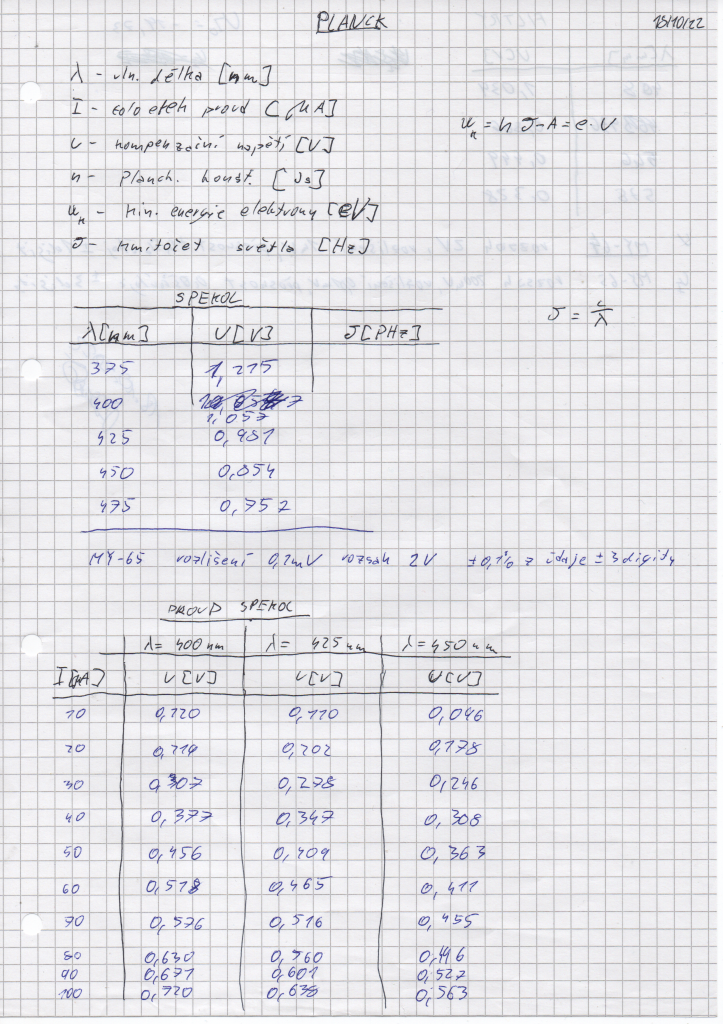
\includegraphics[width=\textwidth]{page1.png}
 \end{minipage}
 \hfil
 \begin{minipage}{0.4\textwidth}
  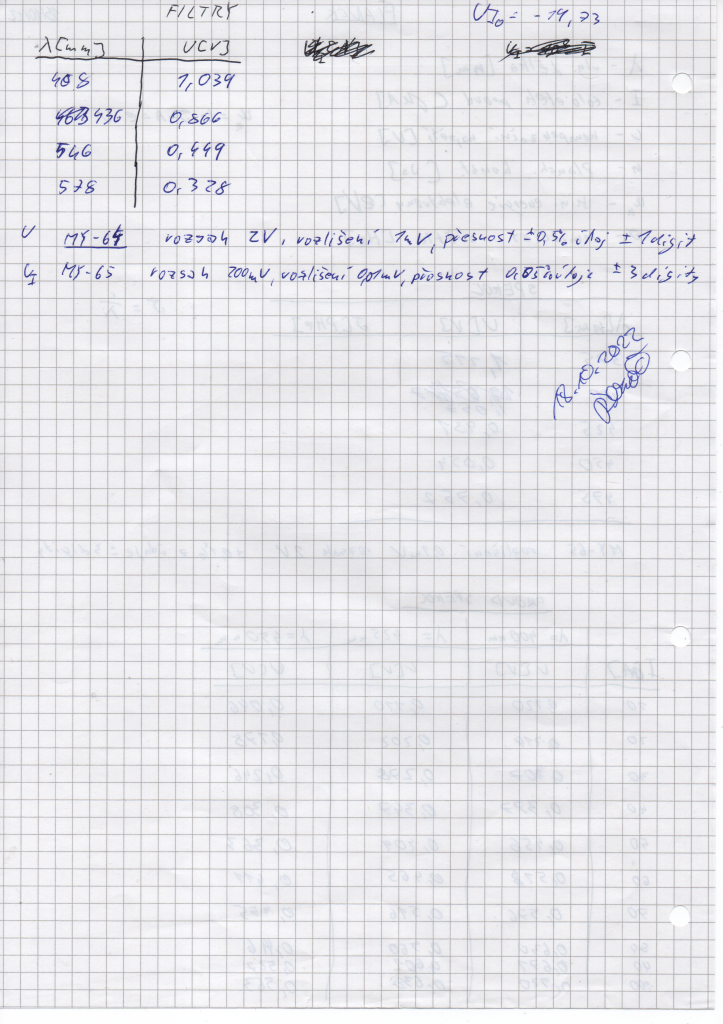
\includegraphics[width=\textwidth]{page2.png}
 \end{minipage}
 \caption{Originální zápis naměřených hodnot}
\end{figure}

\end{document}
